\subsection{Messergebnisse und Auswertung}

\subsubsection{Sägezahnmethode}

\begin{figure}[H]
\begin{center}
  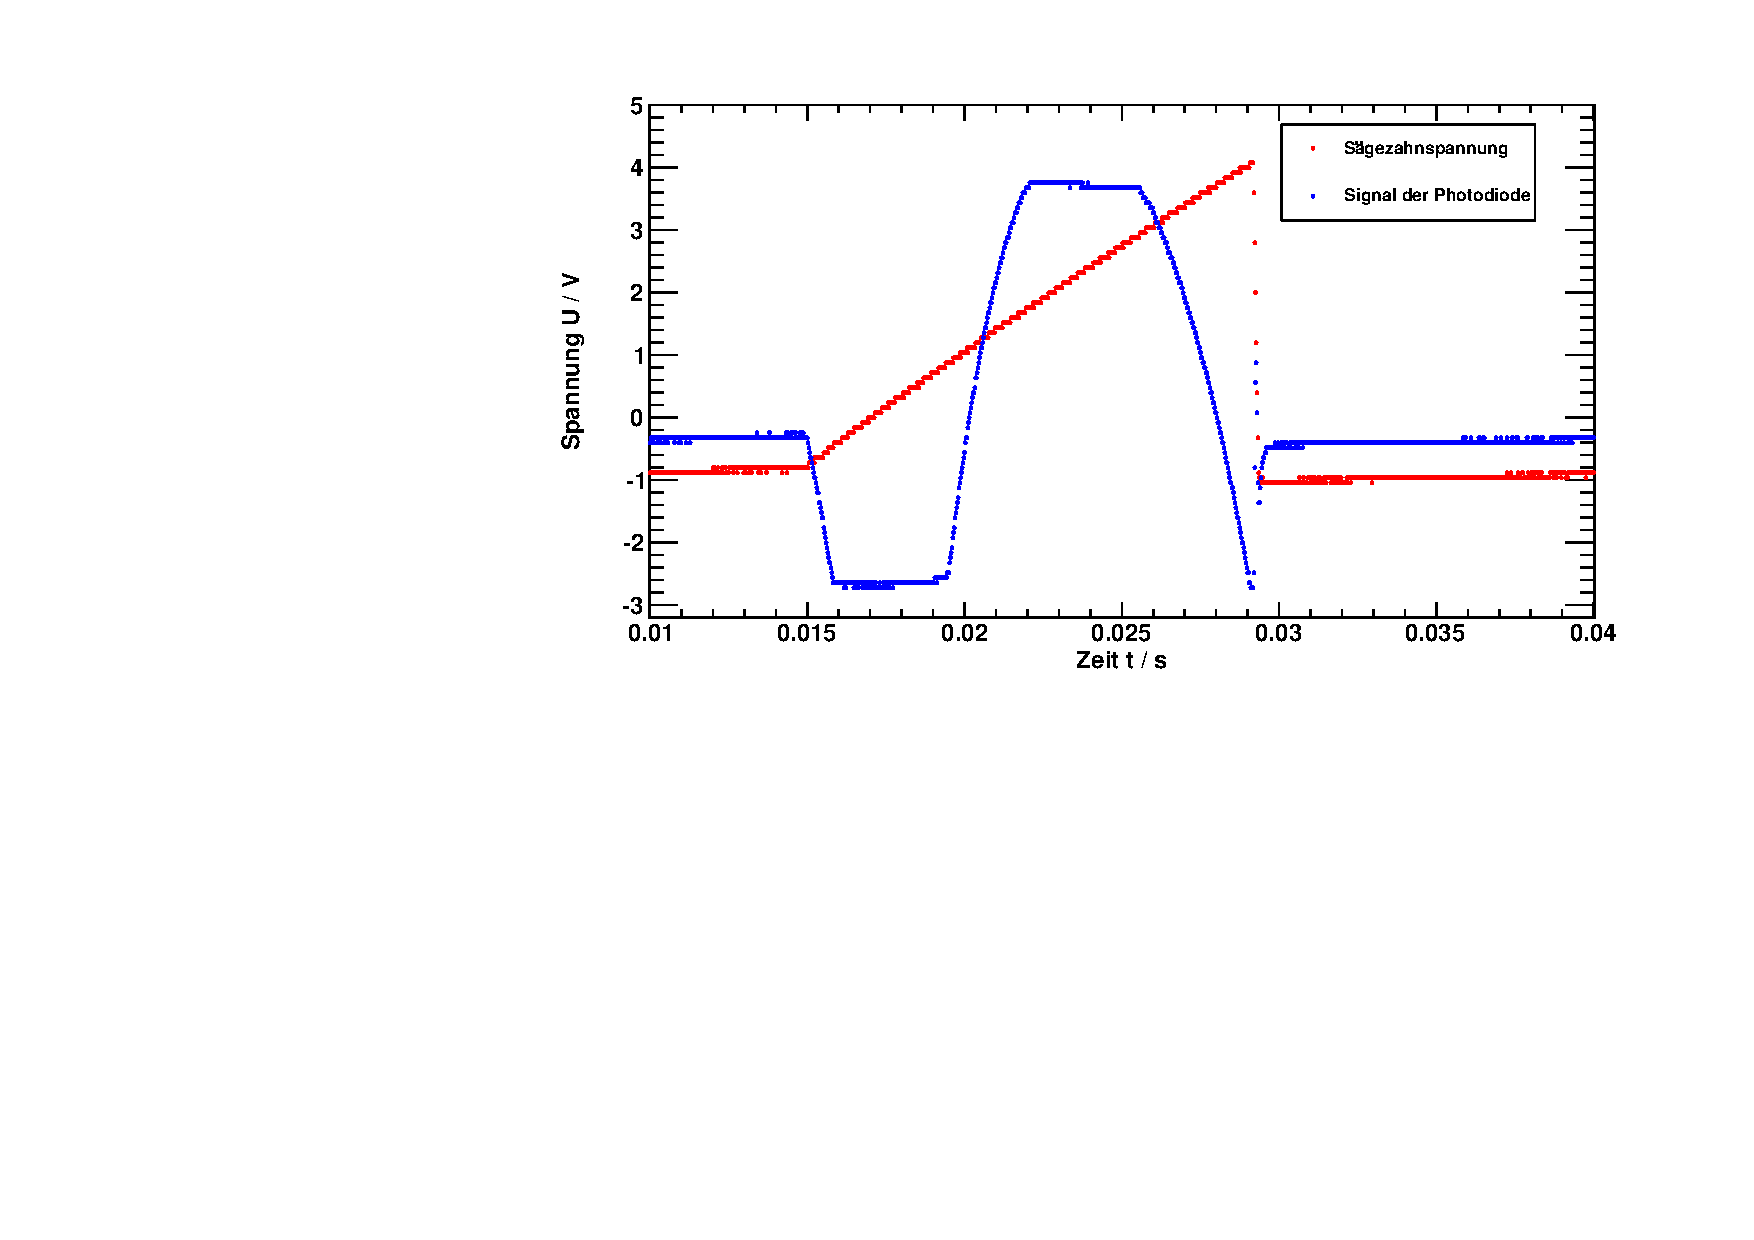
\includegraphics[width=15cm]{../img/pock_saege_winkel0.pdf}
  \caption{Deformiertes Photodiodensignal (blau) bei Einstellung der Polarisationsachse des Analysators in
  Richtung höchster Transmission der Pockelszelle. An der Zelle liegt ein Sägezahnsignal (rot) an.}
  \label{img:pock_saege_winkel0}
\end{center}
\end{figure}

\autoref{img:pock_saege_winkel0} zeigt das Photodiodensignal, wenn der Analysator so eingestellt wird,
wie in der Versuchsanleitung beschrieben, so dass die Amplitude des Photodiodensignals maximiert wird.
Diese Einstellung ist zum Ablesen von Maximum und Minimum des Signals nicht geeignet.
\autoref{img:pock_saege_winkel1}, \autoref{img:pock_saege_winkel2} und \autoref{img:pock_saege_winkel3}
zeigen Messungen mit niedrigerer Amplitude, die für die Auswertung verwendet wurden.

\begin{figure}[H]
\begin{center}
  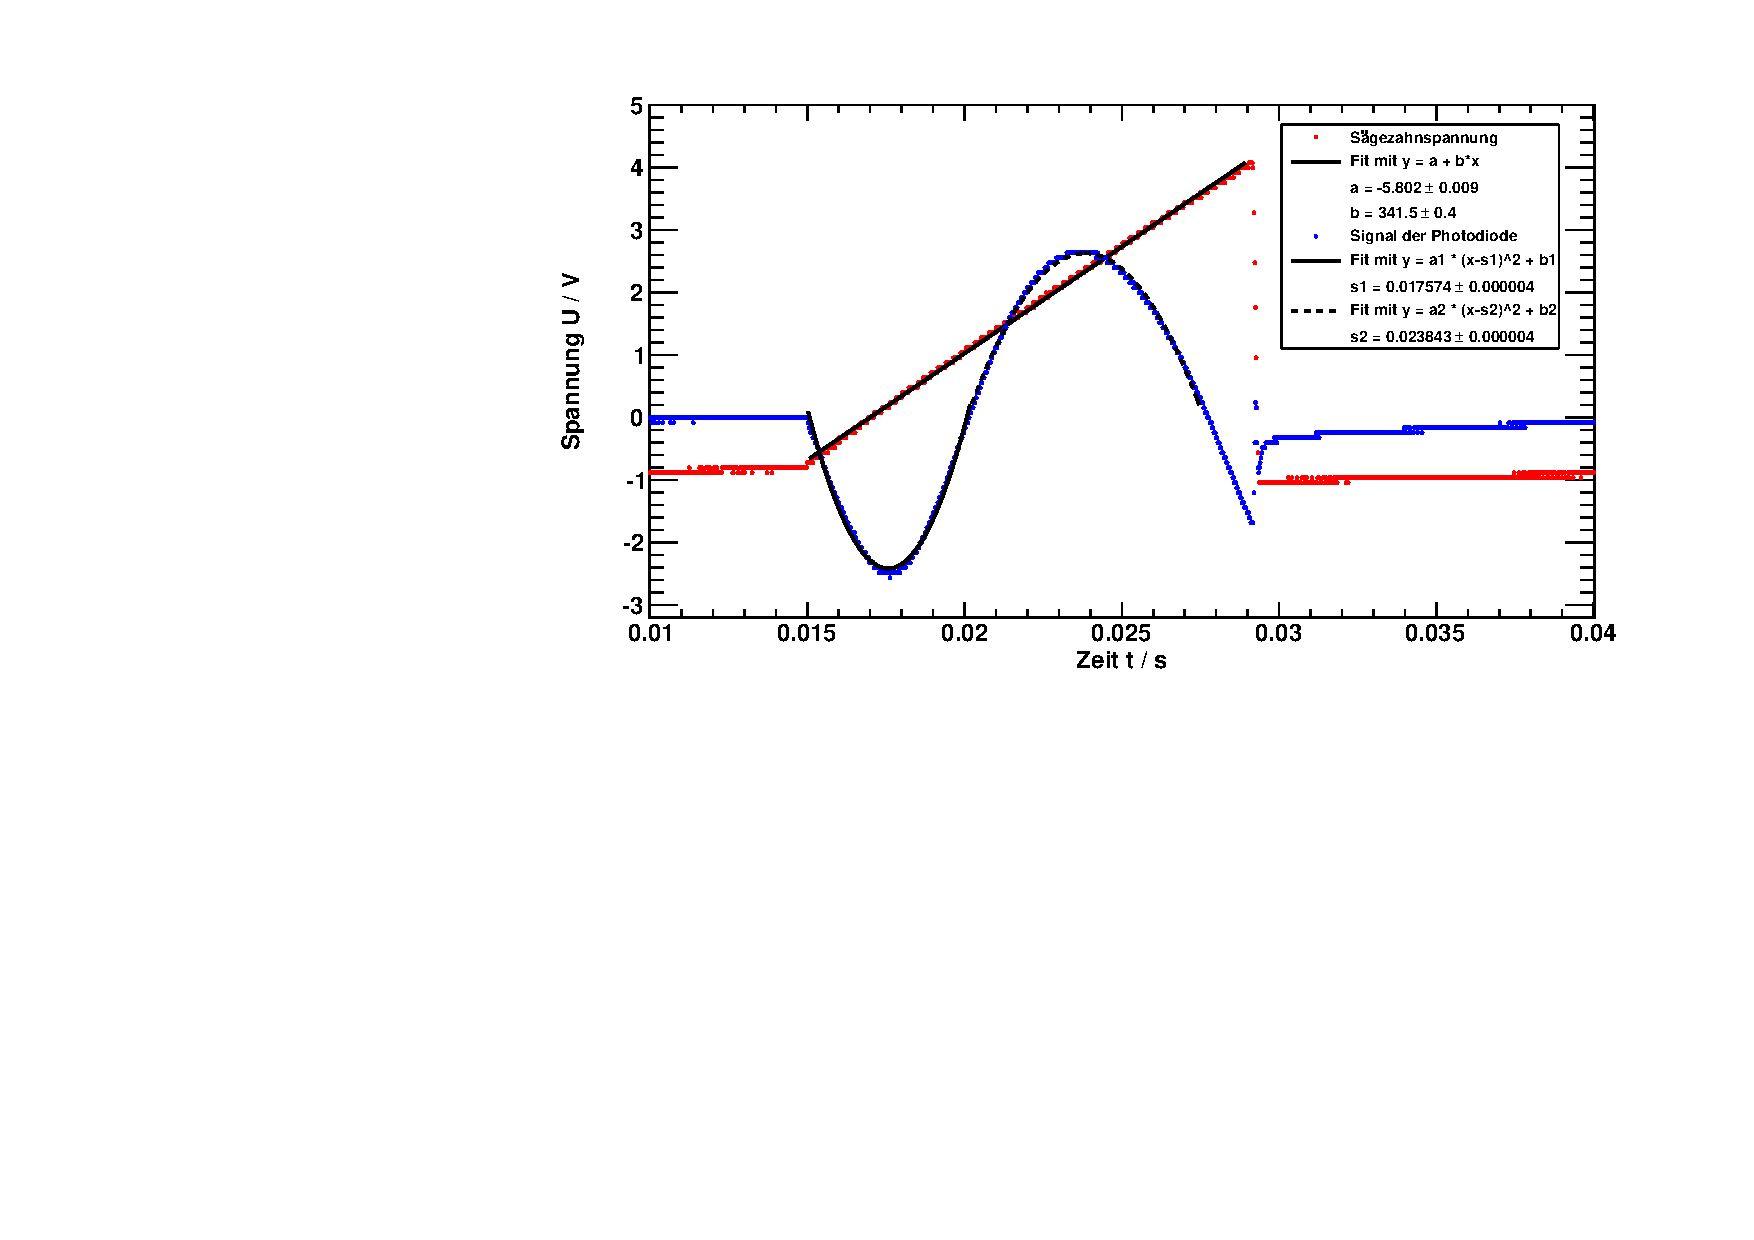
\includegraphics[width=15cm]{../img/pock_saege_winkel1.pdf}
  \caption{1. Messung der Transmission durch den Analysator nach der Pockelszelle mit höchster Signalamplitude
  an der Photodiode (blau). An der Zelle liegt ein Sägezahnsignal (rot) an.}
  \label{img:pock_saege_winkel1}
\end{center}
\end{figure}

\begin{figure}[H]
\begin{center}
  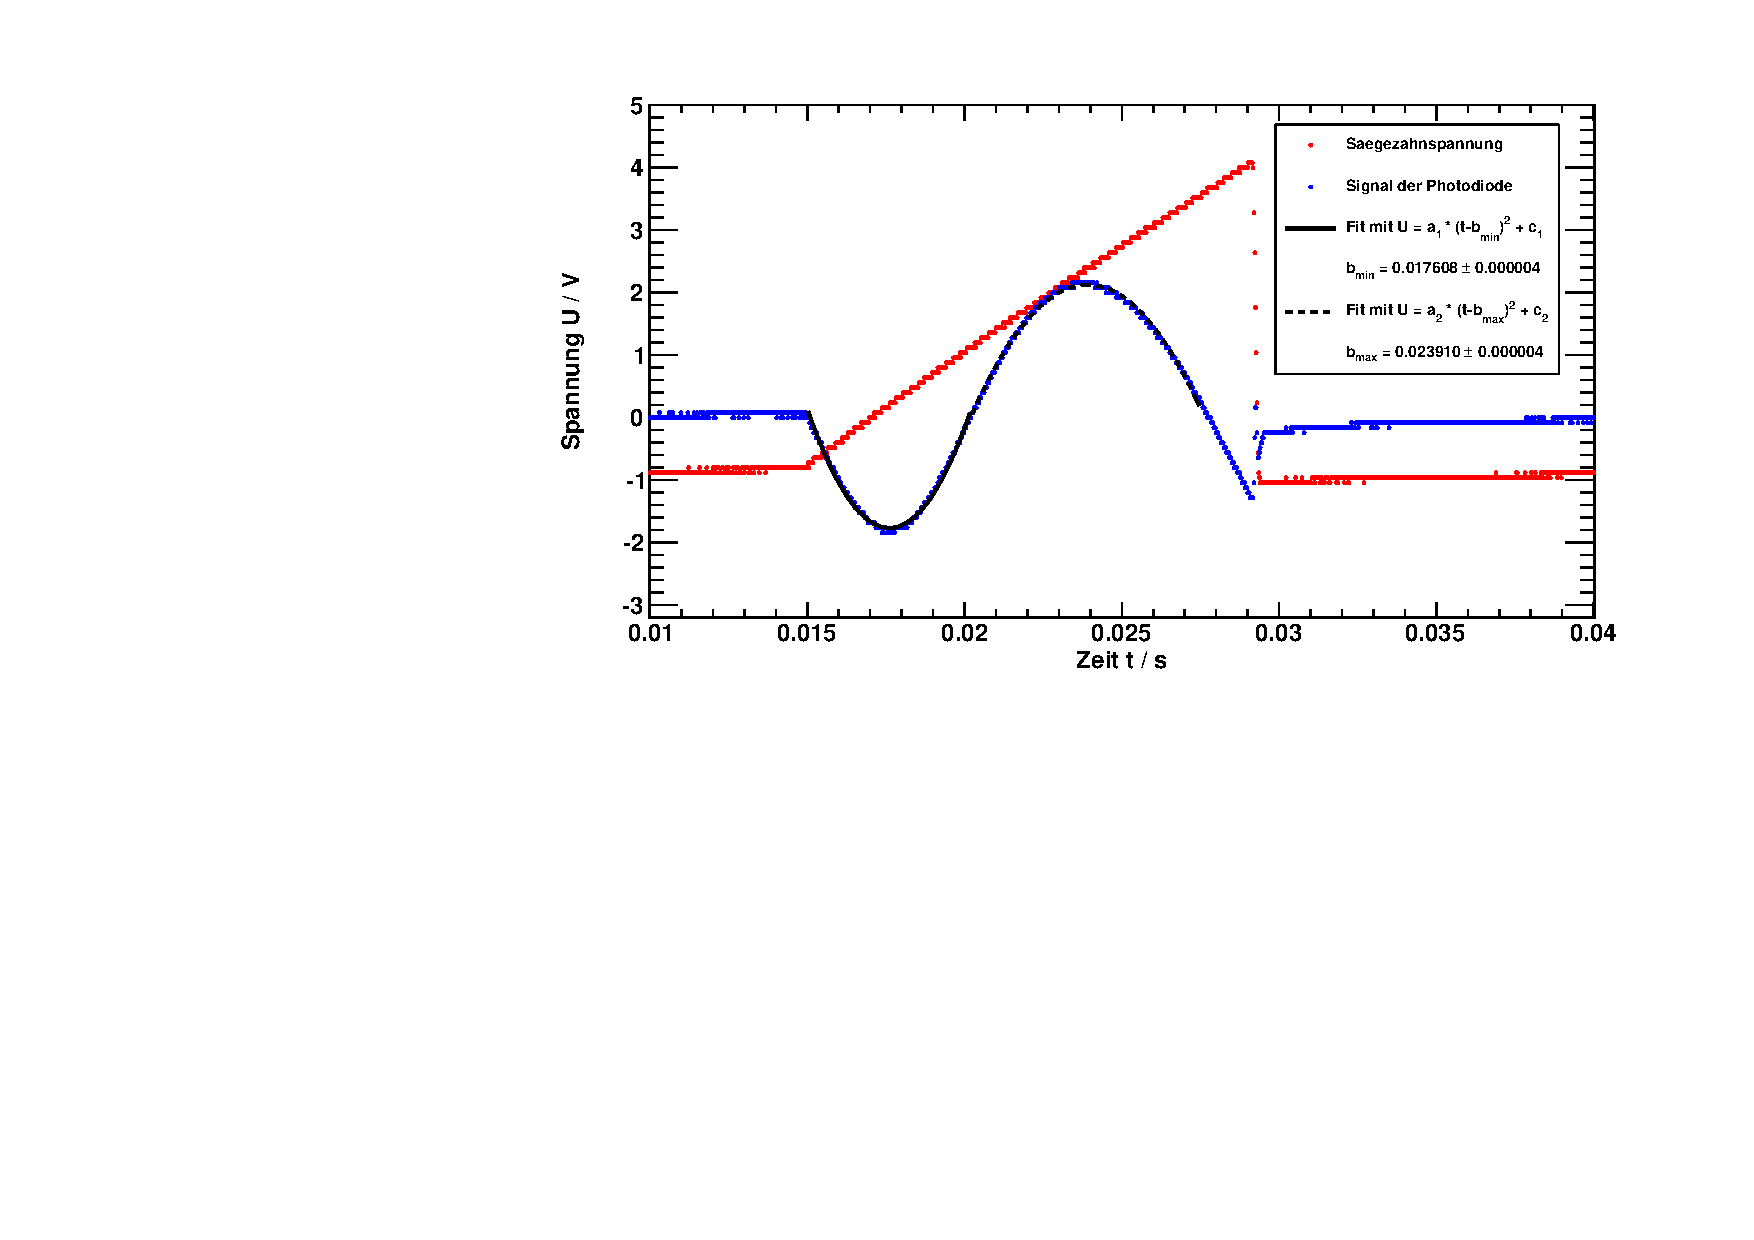
\includegraphics[width=15cm]{../img/pock_saege_winkel2.pdf}
  \caption{2. Messung der Transmission durch den Analysator nach der Pockelszelle mit mittlerer Signalamplitude
  an der Photodiode (blau). An der Zelle liegt ein Sägezahnsignal (rot) an.}
  \label{img:pock_saege_winkel2}
\end{center}
\end{figure}

\begin{figure}[H]
\begin{center}
  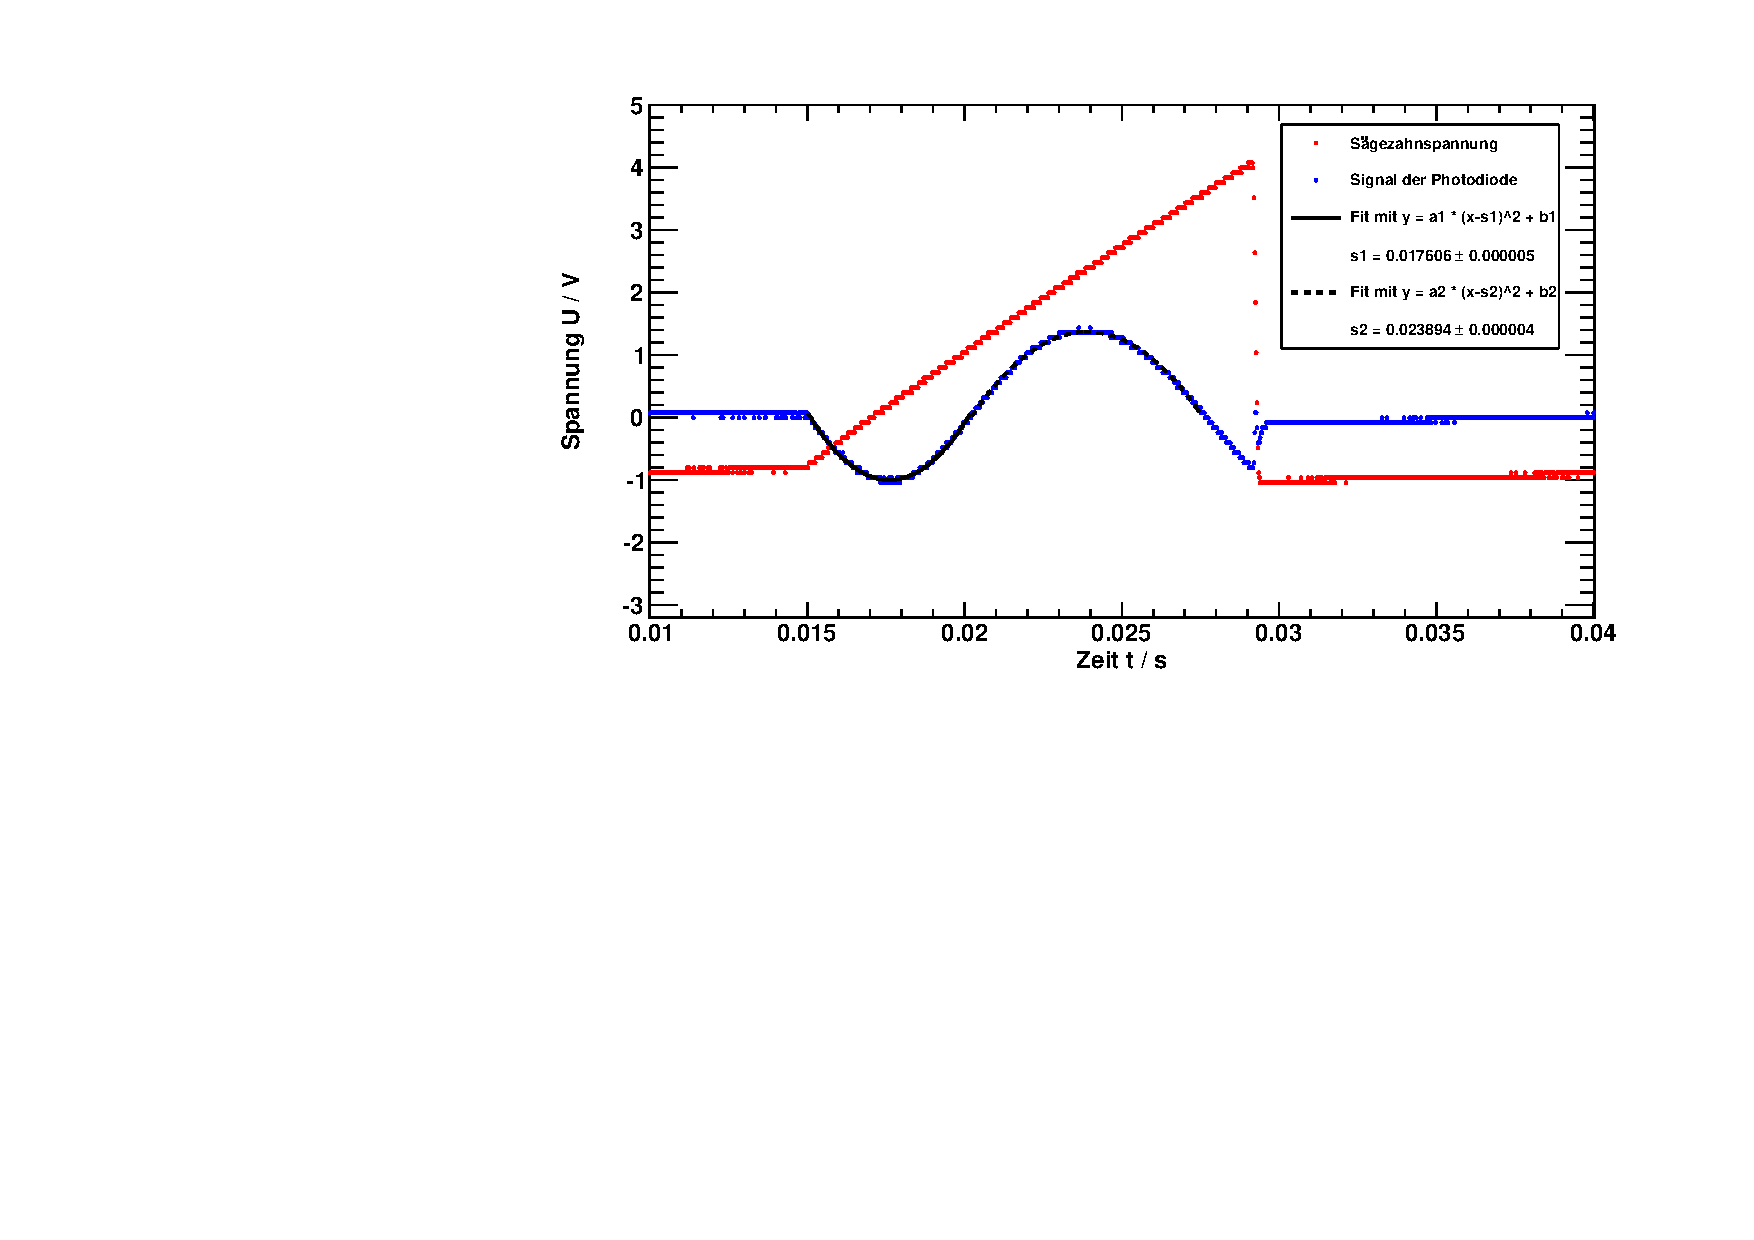
\includegraphics[width=15cm]{../img/pock_saege_winkel3.pdf}
  \caption{3. Messung der Transmission durch den Analysator nach der Pockelszelle mit geringster Signalamplitude
  an der Photodiode (blau). An der Zelle liegt ein Sägezahnsignal (rot) an.}
  \label{img:pock_saege_winkel3}
\end{center}
\end{figure}

In \autoref{tab:minmax} sind die Positionen von Maximum und Minimum für die drei verschiedenen Messungen aufgeführt.
Diese Positionen wurden durch Fits von Parabeln (mit den Fitparametern $a$, $b$ und $c$) an die Messdaten gewonnen:
\begin{equation}
  U = a \cdot (t-b)^2 + c
\end{equation}
Minimum und Maximum wurden hier mit separaten Parabeln gefittet,
weil das Signal offensichtlich kein Sinus ist und ein sinusförmiger Fit keine gute Beschreibung liefert.
Der Parameter $b$ ist die Position des Extremums auf der x-Achse, die für die weitere Auswertung relevant ist.\\
Aus der Position des Maximums $b_{\text{max}}$ und der des Minimums $b_{\text{min}}$
wurde die Differenz $\Delta b$ gebildet:
\begin{equation}
  \Delta b = b_{\text{max}} - b_{\text{min}} \ , \qquad s_{\Delta b} = \sqrt{s_{b_{\text{max}}}^2 + s_{b_{\text{min}}}^2}
\end{equation}
Auch die drei Werte für $\Delta b$ sind in \autoref{tab:minmax} aufgeführt.
\begin{table}[H]
\caption{Position von Maximum und Minimum auf der x-Achse und Positionsdifferenz für die
drei Messungen.}
\begin{center}
\begin{tabular}{|c|c|c|c|c|c|c|}
  \hline
 Messung		& $b_{\text{min}}$ / s 	& $s_{b_{\text{min}}}$ / s 	& $b_{\text{max}}$ / s 	& $s_{b_{\text{max}}}$ / s 	& $\Delta b$ / s 	& $s_{\Delta b}$ / s \\ \hline  
 1 				& 0.017574      		& 0.000004     				& 0.023843   			& 0.000004        			& 0.006269   		& 0.000006       \\ \hline  
 2   		  	& 0.017608       		& 0.000004     				& 0.023910     			& 0.000004        			& 0.006302      	& 0.000005       \\ \hline  
 3 	    		& 0.017606       		& 0.000005     				& 0.023894    			& 0.000004       			& 0.006288    		& 0.000006      \\ \hline   
 
\end{tabular}
\end{center}
\label{tab:minmax}
\end{table}
Im Experiment wurde die Amplitudenabhängigkeit der Messwerte untersucht.
Es ist kein signifikanter Trend erkennbar; die Werte für $\Delta b$ stimmen im 3-\textsigma -Intervall
überein. Dies entspricht unserer Erwartung, da es keinen Grund für eine Amplitudenabhängigkeit
der Position der Extrema gibt.
Deshalb erscheint es gerechtfertigt,
den gewichteten Mittelwert $\overline{\Delta b}$ aus den drei Werten zu bilden. Man erhält
\begin{equation}
  \overline{\Delta b} = (0.006287 \pm 0.000003)\,\text{s}
\end{equation}
\\[\baselineskip]
Die Steigung der Sägezahnfunktion (rote Kurve auf den Abbildungen) wird mit einem Steigungsdreieck abgeschätzt.
Die Positionen der Ecken des Dreiecks
(Spannung am Einsatzpunkt $U_E$, Spannung am Maximum $U_M$, Einsatzzeitpunkt $t_E$ und Maximumszeitpunkt $t_M$)
befinden sich in \autoref{tab:steigungsdreieck}.
\begin{table}[H]
\caption{Messwerte zur Berechnung der Steigung der Sägezahnfunktion.}
\begin{center}
\begin{tabular}{|c|c|c|c|c|}
  \hline
   				& $U$ / V 	& $s_U$ / V & $t$ / s 	& $s_t$ / s \\ \hline  
 Einsatzpunkt 	& -0.8      & 0.1     	& 0.0149   	& 0.0002       \\ \hline  
 Maximum     	& 4.1      	& 0.1     	& 0.0291    & 0.0002       \\ \hline   
 
\end{tabular}
\end{center}
\label{tab:steigungsdreieck}
\end{table}
Man erhält mit den Messwerten für die Steigung der Sägezahnfunktion $m_s$:
\begin{equation}
  m_s = \frac{U_M-U_E}{t_M-t_E} = 345 \,\frac{\text{V}}{\text{s}}
\end{equation}
Für den Fehler darauf folgt mit dem Gaußschen Fehlerfortpflanzungsgesetz
\begin{equation}
  s_{m_s}=\sqrt{\frac{(t_E-t_M)^2 \left(s_{U_E}^2+s_{U_M}^2\right)+(U_E-U_M)^2 \left(s_{t_E}^2+s_{t_M}^2\right)}{(t_E-t_M)^4}}
  =12\,\frac{\text{V}}{\text{s}}
\end{equation}
Die Steigung der Spannung, die an der Pockelszelle anliegt, ist allerdings noch ungefähr um den Faktor 100 höher,
da das Oszilloskop über einen Spannungsteiler mit der Pockelszelle verbunden ist.
Der genaue Dämpfungsfaktor der Schaltung ist aber nicht bekannt und kann nur grob abgeschätzt werden.\\
Wir gehen davon aus, dass während des Sägezahnimpulses
die Spannung an der Zelle von $U_0$ = 0\,V auf $U_1$ = 500\,V steigt,
so wie es im Aufbau vorgesehen ist.
Da wir diese Annahme aber nicht überprüfen können,
die Sägezahnspannung eine leichte Drift zeigt, wo sie konstant 0 sein sollte
und außerdem das nicht-sinusförmige
Signal an der Fotodiode dafür spricht, dass der Aufbau nicht optimal arbeitet
(es ist zum Beispiel an den Einfluss von Kapazitäten zu denken,
die das Sägezahnsignal in der Zelle verformen können),
nehmen wir auf beide Werte einen hohen Fehler von $s_{U_{0,1}}$ = 50\,V an.
Man erhält dann für den Verstärkungsfaktor $A$
\begin{equation}
  A=\frac{U_1-U_0}{U_M-U_E}=102
\end{equation}
und für seinen Fehler
\begin{equation}
  s_A=\sqrt{\frac{(U_0-U_1)^2 \cdot \left(s_{U_E}^2+s_{U_M}^2\right)+(U_E-U_M)^2 \cdot \left(s_{U_0}^2+s_{U_1}^2\right)}{(U_E-U_M)^4}}
  =15
\end{equation}
Nun kann die Halbwellenspannung $U_{\lambda / 2}$ berechnet werden:
\begin{equation}
  U_{\lambda / 2}  = \overline{\Delta b} \cdot m_s \cdot A = 221\,\text{V}
\end{equation}
Für den Fehler $s_{U_{\lambda / 2}}$ gilt
\begin{equation}
  s_{U_{\lambda / 2}} = U_{\lambda / 2} \cdot \sqrt{\left(\frac{s_{\overline{\Delta b}}}{\overline{\Delta b}}\right)^2+\left(\frac{s_{m_s}}{m_s}\right)^2+\left(\frac{s_{A}}{A_{\,}}\right)^2}
  = 33 \,\text{V}
\end{equation}
Aufgrund des ungenauen Messverfahrens hat das Ergebnis für die Halbwellenspannung
\begin{equation}
  U_{\lambda / 2}  = (22 \pm 3) \cdot 10^1\,\text{V}
\end{equation}
einen relativ großen Fehler. \\
Der \emph{elektrooptische Koeffizient} $r_41$ lässt sich nun mit \autoref{eq:r41} bestimmen:
\begin{equation}
  r_{41} = (25 \pm 4)\, \frac{\text{pm}}{\text{V}}
\end{equation}
Der Herstellerwert bei $21^\circ\,$C 
\begin{equation}
  r_{41}^{\text{Herst.}} = 23.4 \, \frac{\text{pm}}{\text{V}}
\end{equation} 
liegt innerhalb des $1$-$\sigma$-Intervalls unseres Messwerts, was jedoch auf den großen Fehler zurückzuführen ist.\\
Im nächsten Abschnitt wird ein genaueres Messverfahren vorgestellt.
\subsubsection{Modulierte Gleichspannung}
Von jedem Spannungswertepaar wird die Differenz berechnet. 
Der Fehler auf eine Einzelmessung beträgt $s_U = 1$\,V.\footnote{Geschätzter Ablese- / Einstellfehler.}
\begin{equation}
  U = U_{\text{pos}} - U_{\text{neg}}, \qquad s_U = \sqrt{2} \cdot s_U
\end{equation}
Es wird dann über alle Spannungen (Anzahl $N$) gemittelt.
\begin{equation}
  \bar{U} = \frac{1}{N} \sum_{i=1}^{N} U_i, \qquad s_{\bar{U}} = \frac{s_U}{\sqrt{N}}
\end{equation}
Mit der Spannung $\bar{U}$ als Halbwellenspannung und \autoref{eq:r41} wird nun der \emph{elektrooptische Koeffizient} für beide Frequenzen bestimmt:
\begin{equation}
  \begin{split}
    r_{41,\, 1\,\text{kHz}}  &= (22.54 \pm 0.05) \, \frac{\text{pm}}{\text{V}} \\
    r_{41,\, 10\,\text{kHz}} &= (22.50 \pm 0.05) \, \frac{\text{pm}}{\text{V}} 
  \end{split}
\end{equation}
Wie erwartet, ist der \emph{elektrooptische Koeffizient} nicht von der Frequenz der verwendeten Spannung abhängig. Aus den zwei Werten wird 
nun noch ein gewichteter Mittelwert gebildet\footnote{Es wird hier mit den genauen Werten gerechnet, nicht den gerundeten.}:
\begin{equation}
  r_{41} = (22.52 \pm 0.04) \, \frac{\text{pm}}{\text{V}}
\end{equation}
Dieser Wert ist nun sehr viel genauer als der mit der Sägezahnmethode bestimmte Wert und stimmt nicht mehr mit dem Wert des Herstellers überein.
\begin{equation}
  r_{41}^{\text{Herst.}} = 23.4 \, \frac{\text{pm}}{\text{V}}
\end{equation}
Dies liegt daran, dass der \emph{elektrooptische Koeffizient} temperaturabhängig ist.